\documentclass{report}

\usepackage{graphicx} % Lets us use images
%\usepackage[acronym]{glossaries} % Lets us use acronyms
\usepackage{multicol}
\usepackage{subcaption}
\usepackage[fleqn]{amsmath}

\author{Charles Pittman}
\title{ELEC-311\\ Project 4\\ Synchronous Design}
\date{December 5, 2013}

%\loadglsentries{acronyms} % Actually loads 'acronyms.tex'
%\makeglossaries

\begin{document}

\maketitle % Inserts title, author, and date from above

%\pagebreak

% Number the enumerate environment (unordered lists) by letter:
%\renewcommand{\labelenumi}{\alph{enumi}.}

\section*{Objective}

% Multiple objectives:
\begin{itemize}
\item Design and test a synchronous sequential circuit which implements a 2-bit binary counter.
\item Describe the circuit using VHDL.
\end{itemize}

 \begin{figure}[hbtp]
   \centering
   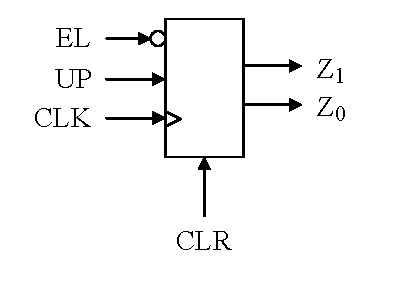
\includegraphics[width=0.5\textwidth]{drawing}
   \caption{\label{fig:counter} 2-bit binary counter}
 \end{figure}

\section*{Discussion}

Figure~\ref{fig:counter} shows a block diagram of the 2-bit binary counter to be implemented.  It takes four inputs: $E_L$, $U_P$, $C_{LK}$, and $C_{LR}$; and the present state is shown by a 2-bit binary number ($Z_1Z_0$).  Since the output (which indicates present state) is only two bits, the circuit can have only four states.  The $U_P$ (active-high) control selects the counter's direction: count up when high; count down when low.  $E_L$ (active-low enable) and $C_{LK}$ (rising-edge triggered) determine when state changes are normally permitted: only when $C_{LK}$ changes low-high while $E_L = 0$.  The only exception to this is $C_{LR}$ (active-high asynchronous clear) signal, which immediately sets the count to 0.

The circuit's regular behavior (i.e. without the asynchronous clear signal) is shown in Table~\ref{tab:trans}.  The sums of minterms in columns $Q_1^+$ and $Q_0^+$ were then used to develop the next-state equations.  Two Karnaugh maps were used (not pictured) to minimize the equations:
%
%\begin{subequations}
%D_1(E_L,U_P,Q_1,Q_0)\nonumber\\
\begin{align}
\label{q1}
  Q_1^+ &=  \sum_m(0,3,5,6,10,11,14,15) \nonumber\\
  &= E_L'U_P'Q_1'Q_0' + U_P'Q_1Q_0 + E_L'U_PQ_1'Q_0 + U_PQ_1Q_0' + E_LQ_1
\end{align}
%
\begin{align}
  \label{eq:D2}
  Q_0^+ &= \sum_m(0,2,4,6,9,11,13,15) \nonumber \\
  &= E_L'Q_0' + E_LQ_0
\end{align}
%\end{subequations}

\begin{table}[hbtp]
  \centering
  \begin{tabular}{c|cc|cc|cc|cc}
 & \multicolumn{2}{c|}{Inputs} & \multicolumn{2}{c|}{PS} & \multicolumn{2}{c|}{NS} & \multicolumn{2}{c}{Outputs} \\
mt & $E_L$ & $U_P$ & $Q_1$ & $Q_0$ & $Q_1^+$ & $Q_0^+$ & $Z_1$ & $Z_0$ \\
\hline
0  & 0    & 0    & 0     & 0     & 1       & 1       & 0     & 0     \\
1  & 0    & 0    & 0     & 1     & 0       & 0       & 0     & 1     \\
2  & 0    & 0    & 1     & 0     & 0       & 1       & 1     & 0     \\
3  & 0    & 0    & 1     & 1     & 1       & 0       & 1     & 1     \\
4  & 0    & 1    & 0     & 0     & 0       & 1       & 0     & 0     \\
5  & 0    & 1    & 0     & 1     & 1       & 0       & 0     & 1     \\
6  & 0    & 1    & 1     & 0     & 1       & 1       & 1     & 0     \\
7  & 0    & 1    & 1     & 1     & 0       & 0       & 1     & 1     \\
8  & 1    & 0    & 0     & 0     & 0       & 0       & 0     & 0     \\
9  & 1    & 0    & 0     & 1     & 0       & 1       & 0     & 1     \\
10 & 1    & 0    & 1     & 0     & 1       & 0       & 1     & 0     \\
11 & 1    & 0    & 1     & 1     & 1       & 1       & 1     & 1     \\
12 & 1    & 1    & 0     & 0     & 0       & 0       & 0     & 0     \\
13 & 1    & 1    & 0     & 1     & 0       & 1       & 0     & 1     \\
14 & 1    & 1    & 1     & 0     & 1       & 0       & 1     & 0     \\
15 & 1    & 1    & 1     & 1     & 1       & 1       & 1     & 1     \\
\end{tabular}
  \caption{\label{tab:trans} Transition Table for Figure~\ref{fig:counter}}
\end{table}



\section*{VHDL}
\label{sec:vhdl}

\begin{verbatim}
library IEEE;
use IEEE.STD_LOGIC_1164.all;

library UNISIM;
use UNISIM.VComponents.all;

use work.project4_pkg.all;

entity counter is
  port (EL  : in  std_logic;  -- Active-low enable
        UP  : in  std_logic;  -- Active-high control (count up/down)
        CLK : in  std_logic;  -- Rising-edge trigger clock
        CLR : in  std_logic;  -- Active-high asynchronous clear
        Z   : out std_logic_vector (1 downto 0));  -- 2-bit number
end counter;

architecture Dataflow of counter is
  signal d        : std_logic_vector(1 downto 0);
  signal q        : std_logic_vector(1 downto 0);
  signal slow_clk : std_logic;

begin
  -- q next-state equations
  d(1) <= (not EL and not UP and not q(1) and not q(0)) or
          (not UP and q(1) and q(0)) or
          (not EL and UP and not q(1) and q(0)) or
          (UP and q(1) and not q(0)) or
          (EL and q(1));
  d(0) <= (not EL and not q(0)) or (EL and q(1));

  -- Stretch the clock input for slow_clk
  CDIV : CLK_DIV port map (CLK, slow_clk);

  -- D flip-flops to do the actual switching
  FF1 : FDC port map(q(1), slow_clk, CLR, d(1));
  FF0 : FDC port map(q(0), slow_clk, CLR, d(0));

  Z <= q;  -- Give Z the present state (for output)
end Dataflow;
\end{verbatim}

\end{document}
